\section{Eksisterende løsninger}
\label{sec:existing-solutions}
Det eksisterer i skrivende stund ingen digitale løsninger på dette problemet. 
Derimot finnes det noen mer manuelle løsninger for å unngå at mutre løsner, 
og løsninger for å sjekke stilling på hjulmuttere.
\subsection{NordLock}
NordLock er et selskap som utvikler bolter og mutre som bruker trykk for å forhindre 
at gjengene løsner, og at bolt og mutter glir fra hverandre. NordLock har flere 
produkter, deriblant en underlagsskive \cite{NL-skive}, figur \ref{fig:NL-skive}, med mothaker mot 
utskruingsretning, og en hjulbolt \cite{NL-hjulbolt}, figur 
\ref{fig:NL-hjulbolt}, som er basert på samme prinsipp som 
underlagsskivene, og som dermed, i flg. NordLock, ikke kan løsne av seg selv.
\newline
\begin{figure}[H]
\subfigure[]{
	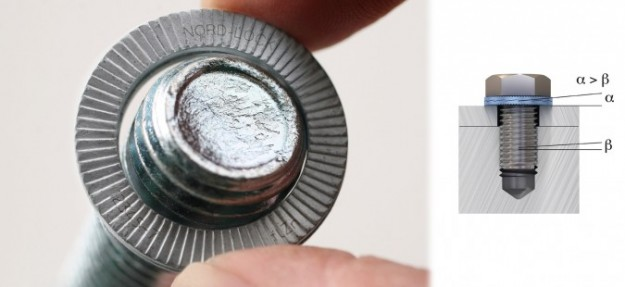
\includegraphics[width=0.5 \textwidth]{images/NL-skive.jpg}
	\label{fig:NL-skive}
	}%
\hfill
\subfigure[]{
	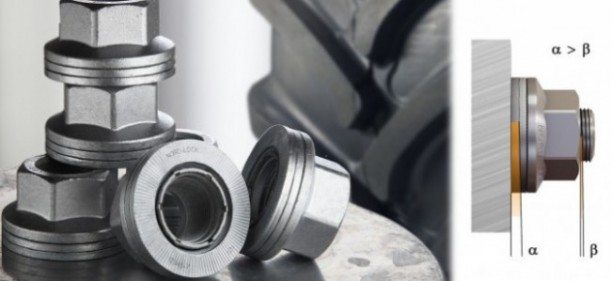
\includegraphics[width=0.5 \textwidth]{images/NL-hjulbolt.jpg}
	\label{fig:NL-hjulbolt}
	}%
\caption{NordLock: \protect{\ref{fig:NL-skive}} underlagsskive, \protect{\ref{fig:NL-hjulbolt}} hjulbolt.}
\end{figure}

Ulempen med NordLock sine produkter, er at man ikke har noen indikasjon på om 
det allikevel har forekommet bevegelse i hjulmutrene. 

\subsection{Checkpoint}
Checkpoint er et selskap som utvikler mer visuelle løsninger på vårt problem.
De har flere produkter for å visualisere endring i stilling på hjulmutter. Den 
viktigste av disse er Checkpoint Original, figur \ref{fig:checkpoint} \cite{checkpoint1}, 
som indikerer dersom hjulmutteren den er festet på har endret posisjon. 
	\newline
	\begin{figure}[H]
		\centering
		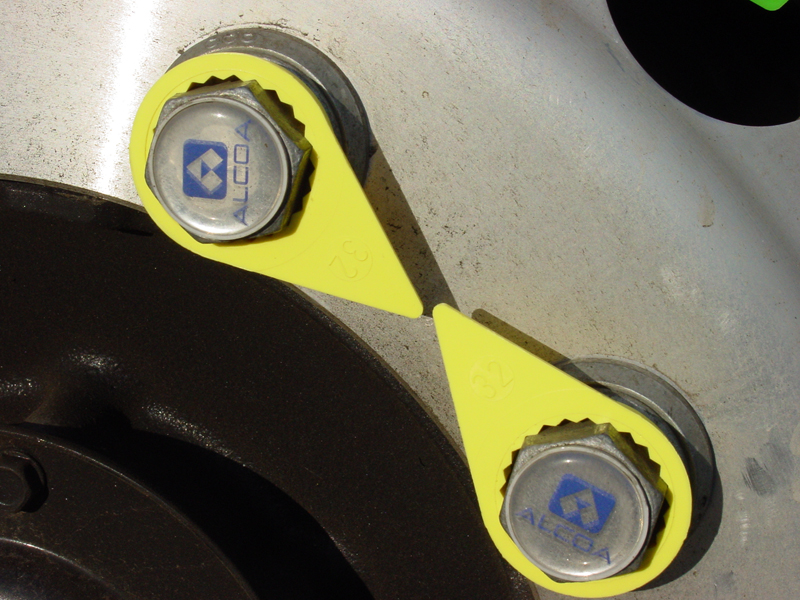
\includegraphics[width=0.50\textwidth]{images/checkpoint-original.jpg}
		\caption{Checkpoint Original viser dersom det er bevegelse i hjulmutter.}
		\label{fig:checkpoint}
	\end{figure}
Ulempen med Checkpoint kontra en digital løsning, er at sjåfør manuelt må gå over 
hvert enkelt hjul for å se etter avvik, og man får ingen sanntidsinformasjon om 
status på hjulmuttrene.

\subsection{Digital visualisering}
Det eksisterer i skrivende stund ingen softwarebaserte visuelle løsninger av dette 
problemet. Figuren nederst til venstre i bildet under viser hvordan  
Polyphony Digital løste visualisering av 
dekkslitasje i sitt spill Gran Turismo 6. \cite{dekkslitasje-GT6} 
	\newline
	\begin{figure}[H]
		\centering
		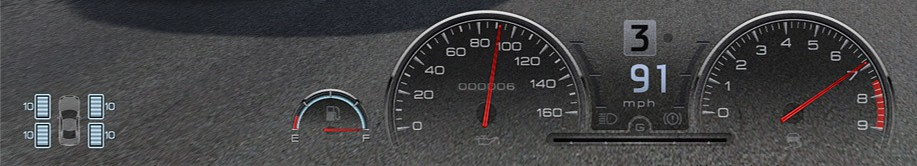
\includegraphics[width=1.00\textwidth]{images/gran-turismo-6-screenshot.jpg}
		\label{fig:GT6}
		\caption{Dekkslitasje visualisert i Gran Turismo 6.}
	\end{figure}
